\title{Assignment 3.1}
\author{
        Pradyot Prakash - 130050008
            \\
        Utkarsh Mall - 130050037
			\\
		Samarth Mishra - 130260018
}
\date{\today}
\documentclass[11pt]{article}
\usepackage[left=2.5cm,top=2cm,right=2.5cm,bottom=2cm,bindingoffset=0.5cm]{geometry}
\usepackage{graphicx}
\usepackage{siunitx}
\usepackage[section]{placeins}
\graphicspath{ {../images/} }
\renewcommand\thesubsection{(\alph{subsection})}
\begin{document}
\maketitle

\subsection{}
RRMSE Between Noisy and Noiseless Image 
$$RRMSE = 0.2612$$

\subsection{}
\hfill \break
\textbf{Quadratic Prior}
\begin{itemize}
	\item Optimal $\alpha$ is $0.0005$
	\item RRMSE ar $\alpha$ is $2.438248e-01$
	\item RRMSE at $0.8\alpha$ is $2.438240e-01$
	\item RRMSE at $1.2\alpha$ is $2.501484e-01$
	\item $\gamma$ does not affects the quadratic prior
\end{itemize}

\hfill \break
\textbf{Huber Prior}
\begin{itemize}
	\item Optimal $\alpha$ is $ 0.00005 $ and $\gamma$ is $0.23$ 
	\item RRMSE ar $\alpha$ and $\gamma$ is $2.368141e-01$
	\item RRMSE at $0.8\alpha$ and $\gamma$ is $2.368141e-01$
	\item RRMSE at $1.2\alpha$ and $\gamma$ is $2.370435e-01$
	\item RRMSE at $\alpha$ and $0.8\gamma$ is $2.372921e-01$
	\item RRMSE at $\alpha$ and $1.2\gamma$ is $2.372365e-01$
\end{itemize}

\hfill \break
\textbf{Discontinuity-adaptive Prior}
\begin{itemize}
	\item Optimal $\alpha$ is $0.000006$ and $\gamma$ is $0.04$ 
	\item RRMSE ar $\alpha$ and $\gamma$ is $1.990510e-01$
	\item RRMSE at $0.8\alpha$ and $\gamma$ is $1.997076e-01$
	\item RRMSE at $1.2\alpha$ and $\gamma$ is $2.003708e-01$
	\item RRMSE at $\alpha$ and $0.8\gamma$ is $1.985012e-01$
	\item RRMSE at $\alpha$ and $1.2\gamma$ is $2.006748e-01$
\end{itemize}

\subsection{}
\begin{figure}[h]
\centering
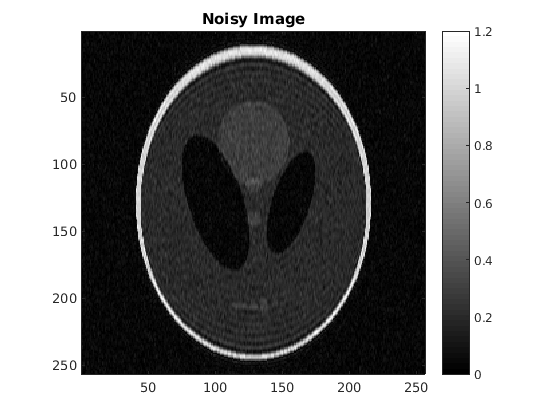
\includegraphics[scale=0.5]{Noisy}
\end{figure}

\begin{figure}[h]
\centering
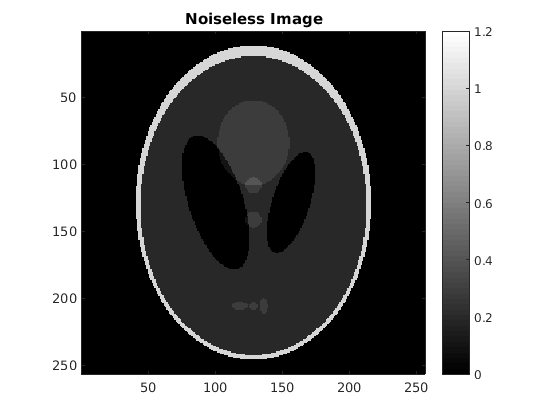
\includegraphics[scale=0.5]{Noiseless}
\end{figure}

\begin{figure}[h]
\centering
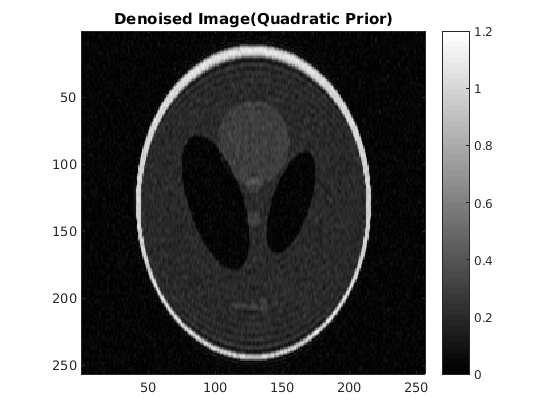
\includegraphics[scale=0.5]{DenoisedQuad}
\end{figure}

\begin{figure}[h]
\centering
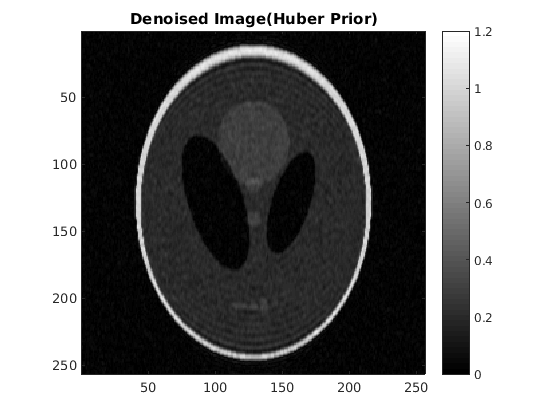
\includegraphics[scale=0.5]{DenoisedHuber}
\end{figure}

\begin{figure}[h]
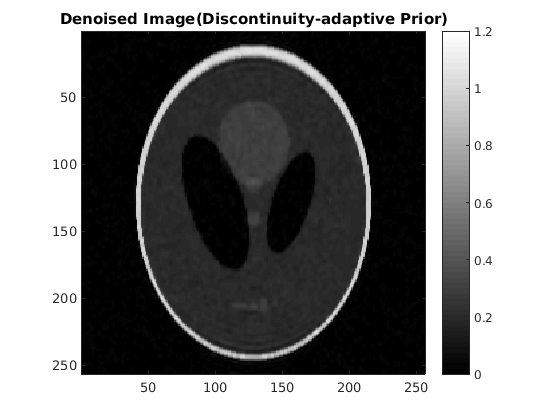
\includegraphics[scale=0.5]{DenoisedDA}
\centering
\end{figure}
\FloatBarrier

\subsection{}
\begin{figure}[h]
\hspace*{-1.5in}
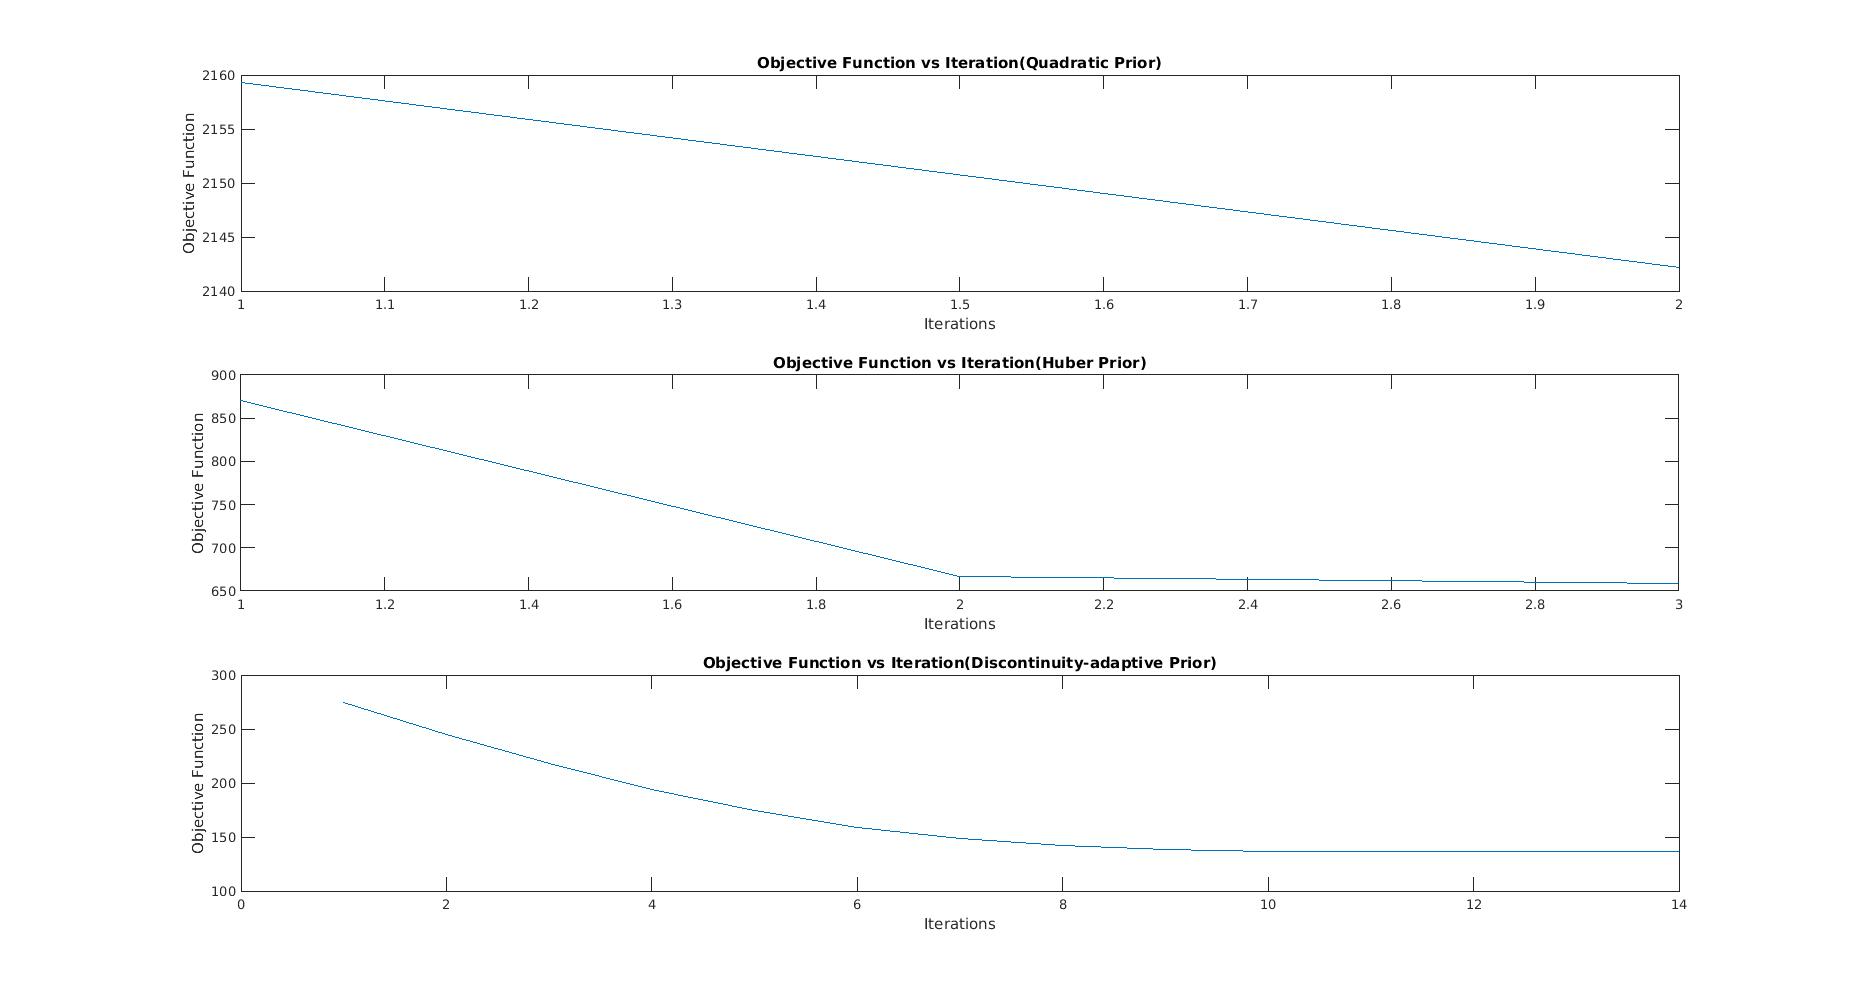
\includegraphics[scale=0.48]{graphs}
\centering
\end{figure}
\FloatBarrier

\end{document}
